\documentclass[12pt]{beamer}

\usepackage[brazil]{babel}
\usepackage[utf8]{inputenc}
\usepackage[T1]{fontenc}
\usepackage{animate}
\usepackage{amsbsy}
\usepackage{amsfonts}
\usepackage{amsmath}
\usepackage{amssymb}
\usepackage{amsthm}
\usepackage[toc,page,title,titletoc]{appendix}
\usepackage{dsfont}
\usepackage{esvect}
\usepackage[labelfont=bf]{caption}
\usepackage{subcaption}
\usepackage{float}
\usepackage[Glenn]{fncychap}%Sonny %Conny %Lenny %Glenn %Renje %Bjarne %Bjornstrup
\usepackage{graphicx}
\usepackage{indentfirst}%Para indentar os paragrafos automáticamente
\usepackage{lipsum}
\usepackage{longtable}
\usepackage{mathtools}
\usepackage{listings}%Inserir codigo do R no latex
\usepackage{multirow}
\usepackage{multicol}
\usepackage{csquotes}
\usepackage[citestyle=authoryear,maxcitenames=2,terseinits=true,natbib=true, style=abnt]{biblatex}
\addbibresource{Referencias.bib}
\usepackage[figuresright]{rotating}
\usepackage{spalign}
\usepackage{pgfplots}
\pgfplotsset{compat=1.17}
\usepackage{tikz}
\usepackage{color, colortbl}
\usepackage{url}
\usepackage{ragged2e}%para justificar o texto dentro de algum ambiente
\definecolor{Gray}{gray}{0.9}
\definecolor{LightCyan}{rgb}{0.88,1,1}


\usepackage[all]{xy}
\usepackage{hyperref,bookmark}
\hypersetup{
  colorlinks=true,
  linkcolor=blue,
  citecolor=red,
  filecolor=blue,
  urlcolor=blue,
}

\usetheme{Madrid}
\usecolortheme[RGB={193,0,0}]{structure}

%\setbeamertemplate{footline}[frame number]
%\setbeamertemplate{footline}[text line]{%
%  \parbox{\linewidth}{\vspace*{-8pt}\hfill\date{}\hfill\insertshortauthor\hfill\insertpagenumber}}
\beamertemplatenavigationsymbolsempty
\renewcommand{\vec}[1]{\mbox{\boldmath$#1$}}
\newtheorem{Teorema}{Teorema}
\newtheorem{Proposicao}{Proposição}
\newtheorem{Definicao}{Definição}
\newtheorem{Corolario}{Corolário}
\newtheorem{Demonstracao}{Demonstração}
\newcommand{\bx}{\ensuremath{\bar{x}}}
\newcommand{\Ho}{\ensuremath{H_{0}}}
\newcommand{\Hi}{\ensuremath{H_{1}}}


\apptocmd{\frame}{}{\justifying}{} % Allow optional arguments after frame.

\title{Estatística Básica}
\author{Prof. Fernando de Souza Bastos\texorpdfstring{\\ fernando.bastos@ufv.br}{}}
\institute{Instituto de Ciências Exatas e Tecnológicas\texorpdfstring{\\ Universidade Federal de Viçosa}{}\texorpdfstring{\\ Campus UFV - Florestal}{}}
\date{}
\newcommand\mytext{Aula 1}
\newcommand\mytextt{Fernando de Souza Bastos}
\newcommand\mytexttt{\url{https://maf105.github.io/}}

\makeatletter
\setbeamertemplate{footline}
{
  \leavevmode%
  \hbox{%
  \begin{beamercolorbox}[wd=.3\paperwidth,ht=2.25ex,dp=1ex,center]{author in head/foot}%
    \usebeamerfont{author in head/foot}\mytext
  \end{beamercolorbox}%
  \begin{beamercolorbox}[wd=.3\paperwidth,ht=2.25ex,dp=1ex,center]{title in head/foot}%
    \usebeamerfont{title in head/foot}\mytextt
  \end{beamercolorbox}%
  \begin{beamercolorbox}[wd=.35\paperwidth,ht=2.25ex,dp=1ex,right]{site in head/foot}%
    \usebeamerfont{site in head/foot}\mytexttt\hspace*{2em}
    \insertframenumber{} / \inserttotalframenumber\hspace*{2ex} 
  \end{beamercolorbox}}%
  \vskip0pt%
}
\makeatother

\providecommand{\arcsin}{} \renewcommand{\arcsin}{\hspace{2pt}\textrm{arcsen}}
\providecommand{\sin}{} \renewcommand{\sin}{\hspace{2pt}\textrm{sen}}
%\newtheorem{Teorema}{Teorema}
%\newtheorem{Proposicao}{Proposição}
%\newtheorem{Definicao}{Definição}
%\newtheorem{Corolario}{Corolário}
%\newtheorem{Demonstracao}{Demonstração}

\titlegraphic{\hspace*{8cm}\href{https://fsbmat-ufv.github.io/}{
\includegraphics[width=2cm]{figs/mylogo.png}}
}

% Layout da pagina
\hypersetup{pdfpagelayout=SinglePage}
\begin{document}
%\SweaveOpts{concordance=TRUE}

\frame{\titlepage}

\begin{frame}{}
\frametitle{\bf Sumário}
\tableofcontents
\end{frame}

\section{Preliminares}
\begin{frame}{}
\frametitle{}
\begin{block}{}
\justifying
Em alguma fase de seu trabalho, o pesquisador depara-se com o problema de analisar e entender um conjunto de dados relevante ao seu particular objeto de estudos. Ele necessitará trabalhar os dados para transformá-los em informações, para compará-los com outros resultados, ou ainda para julgar sua adequação a alguma teoria.
\end{block}
\end{frame}

\begin{frame}{}
\frametitle{}
\begin{block}{}
\justifying
\begin{center}
\Large{\bf{Não Tem Como Escapar dos Dados!}}
\end{center}
\end{block}
\end{frame}

\begin{frame}{}
\frametitle{}
\begin{block}{}
\justifying
\begin{figure}[H]
    \centering
    \caption{Era do Big Data}
    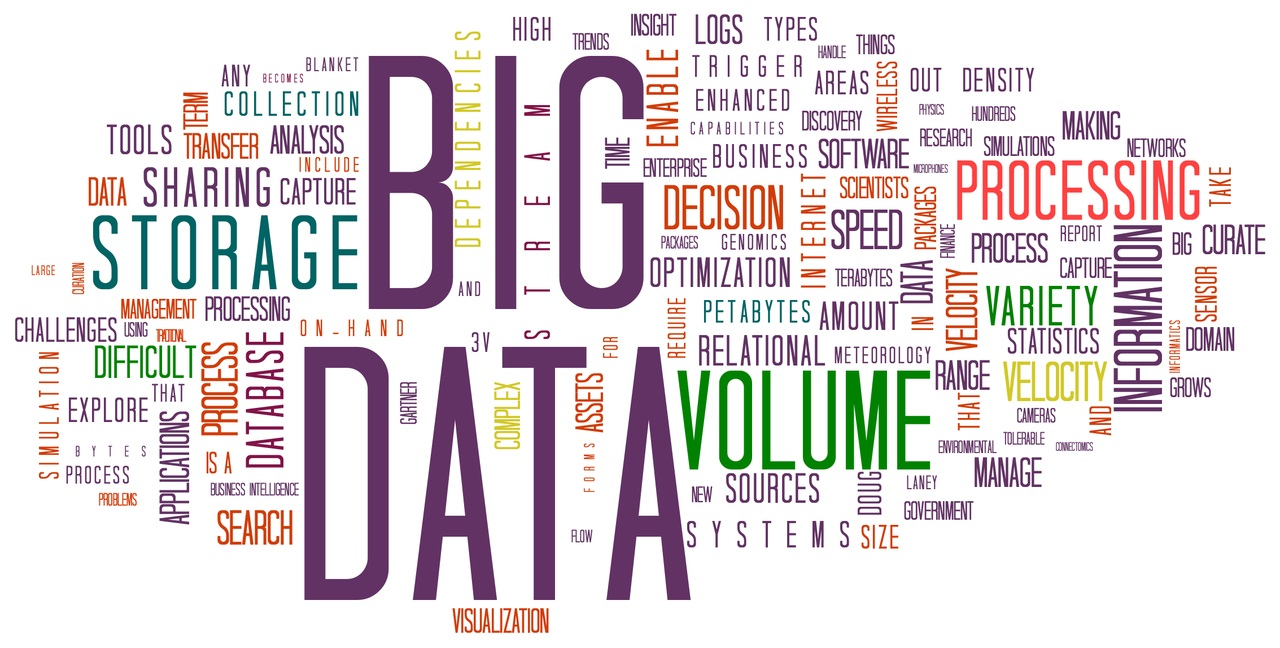
\includegraphics[scale=0.3]{figs/BigData.jpg}
    \subcaption*{\textbf{Fonte:} Revista Exame 2017 \cite{exame17}}
    %\label{figRotulo}
  \end{figure}
\end{block}
\end{frame}

\begin{frame}{}
\frametitle{}
\begin{block}{}
\justifying
\begin{itemize}
\item Google: são mais de 5,5 bilhões de buscas por dia \cite{ardorseo}.\pause
\item \citet{youtube}: mais de 2 bilhões de usuários e são assistidas mais de 1 bilhão de horas de vídeos por dia.\pause
\item Facebook: Há picos de 2,8 bilhões de usuários ativos diariamente \cite{internetstats}.\pause
\item Instagram: Mais de 1 bilhão de usuários, mais de 500 milhões de pessoas usam o \textit{stories} todos os dias \cite{InstagramStats}.\pause
\item WhatsApp: mais de 100 bilhões de mensagens por dia e mais de 2 bilhões de usuários \cite{WhatsappStats}.\pause
\item Twitter: 500 milhões de tweets por dia e 340 milhões de usuários ativos \cite{TwitterStats}.
\end{itemize}
\end{block}
\end{frame}

\begin{frame}{}
\frametitle{}
\begin{block}{}
\justifying
\begin{itemize}
\item Internet: mais de 1,8 bilhões de sites \cite{internetstats2} e 4,6 bilhões de pessoas conectadas \cite{statista}.\pause
\item Telefones celulares: mais de 5,7 bilhões \cite{datareportal}.\pause
\item Dispositivos conectados: serão 50 bilhões em 2030 \cite{statista}.\pause
\item De acordo com \citet{seedscientific}, em 2025, a quantidade de dados gerados a cada dia deve chegar a 463 exabytes ($10^{18} bytes$) globalmente.
\end{itemize}
\end{block}
\end{frame}

\begin{frame}{}
\frametitle{}
\begin{block}{}
\justifying
A IDC (empresa líder em inteligência de mercado e consultoria nas indústrias de tecnologia da informação, telecomunicações e mercados de consumo em massa de tecnologia) estimou, em 2014, que do total de dados no mundo, $22\%$ contêm informação útil. E apenas $5\%$ foram analisados e utilizados de alguma forma \cite{exame14}.
\end{block}
\end{frame}

\begin{frame}{}
\frametitle{}
\begin{block}{}
\justifying
Como processar tanta informação? Como gerar informação a partir dos dados? Essa não é uma tarefa fácil, é necessário, anos de estudo e variadas competências, Estatística, Matemática, Ciência da Computação e diversas outras. Mas o profissional que tem conhecimento estatístico e sabe avaliar processos ou prever possíveis resultados a partir da analise de bancos de dados é um dos profissionais mais requisitados na atualidade e recebe os maiores salários!
\end{block}
\end{frame}

\begin{frame}{}
\frametitle{}
\begin{block}{Engenheiro ou Cientista de Dados}
\begin{itemize}
\justifying
\item {\bf O que faz:} combina habilidades em negócios e estatística. É o profissional responsável por solucionar problemas do negócio com técnicas de orientação a dados, bem como detectar tendências que podem ajudar nos resultados de uma empresa.
\item {\bf Perfil:} qualificações estatísticas, matemáticas e curiosidade para fazer descobertas em big data.
\item {\bf Salário:} R\$ 6 mil a R\$ 14 mil\\
\end{itemize}
{\bf Fonte:} \url{https://www.salario.com.br/profissao/cientista-de-dados-data-scientist/}, visitado em junho de 2021.
\end{block}
\end{frame}


\begin{frame}{}
\frametitle{}
\begin{block}{}
\justifying
Você precisa ser especialista em Estatística ou Matemática ou mesmo ter feito uma graduação nestas áreas? \pause A resposta é {\bf não}. \pause Apesar dessas áreas permitirem uma compreensão mais abrangente, é possível aprender os conceitos necessários para o que você precisa e aplica-los ao longo da sua jornada de aprendizagem. \textbf{Você não precisa aprender todos os tópicos relacionados à Estatística ou Matemática}.

{\bf Fonte:} \url{http://datascienceacademy.com.br/blog/cientista-de-dados-por-onde-comecar-em-8-passos/}
\end{block}
\end{frame}

\section{Introdução}
\begin{frame}{}
\frametitle{Introdução}
\begin{block}{}
\justifying
Estatística é a ciência que nos ajuda a tomar decisões e tirar conclusões na presença de variabilidade. A estatística é uma maneira de raciocinar que pode ajudar você a tomar decisões mais bem fundamentadas. A estatística ajuda você a solucionar problemas que envolvem decisões que estão baseadas em dados que tenham sido coletados.
\end{block}
\pause
\begin{block}{}
\justifying
Vamos seguir uma \textbf{regra} fundamental:
``A Estatística deve simplificar, não complicar a interpretação dos dados''.
\end{block}
\end{frame}

\begin{frame}{}
\frametitle{Introdução}
\begin{block}{}
\justifying
Ressalto que a Estatística é a ciência que ensina a ``ESCUTAR'' os dados, não é uma ciência para provar alguma coisa em relação ao que você deseja que os dados digam!
\end{block}
\pause
\begin{block}{}
\justifying
A estatística é a arte de torturar os números até que eles confessem!
*Como mentir com estatísticas \cite{huff2016mentir} (reedição de 1954)
\end{block}
\pause
\begin{block}{}
\justifying
O pensamento estatístico será um dia tão necessário para uma cidadania eficiente quanto a capacidade de ler e escrever! Citação do discurso presidencial em 1951 do estatístico matemático Samuel S. Wilks (1906 - 1964) à American Statistical Association encontrado em ``JASA'', vol. 46, No. 253., pp. 1-18. 
\end{block}
\pause
\begin{block}{}
\justifying
Leiam também \citet{super16}!
\end{block}
\end{frame}

\begin{frame}{}
\frametitle{Introdução}
\begin{block}{}
\justifying
Na primeira parte deste curso estaremos interessados em:
\begin{itemize}
\item Reduzir ou organizar, limpar e resumir, analisar e interpretar dados!
\end{itemize}
\end{block}
\pause
\begin{block}{}
\justifying
Essa será a parte inicial do curso denominada Análise exploratória de dados (AED). Queremos nessa fase obter dos dados a maior
quantidade possível de informação, para indicar modelos plausíveis a serem utilizados
na inferência estatística.
\end{block}
\end{frame}

\begin{frame}{}
\frametitle{Introdução}
\begin{block}{}
\justifying
Vamos aprender e calcular algumas medidas de posição e de variabilidade. E aprender técnicas gráficas para a análise exploratória de dados. 
\end{block}
\end{frame}

\begin{frame}{}
\frametitle{Modelos}
\begin{block}{}
\justifying
Vamos utilizar os livros:
\begin{itemize}
    \item \citetitle{morettin2017estatistica} dos autores Wilton de Oliveira Bussab e Pedro Alberto Morettin;
    \item \citetitle{eric} dos autores Eric Batista Ferreira e Marcelo Silva de Oliveira.
\end{itemize}
\end{block}
\end{frame}


\begin{frame}[allowframebreaks]
\frametitle{\bf Referências}
\printbibliography
\end{frame}


\end{document}
